\documentclass[12pt]{article} % use larger type; default would be 10pt
\usepackage[utf8]{inputenc} % set input encoding (not needed with XeLaTeX)

%%% PAGE DIMENSIONS
\usepackage{geometry} % to change the page dimensions
\geometry{a4paper} % or letterpaper (US) or a5paper or....
\geometry{margin=2cm} % or letterpaper (US) or a5paper or....

\usepackage{graphicx} % support the \includegraphics command and options
\usepackage[parfill]{parskip} % Activate to begin paragraphs with an empty line rather than an indent
\usepackage{times} % for Times Roman default font

%%% PACKAGES
\usepackage{booktabs} % for much better looking tables
\usepackage{array} % for better arrays (eg matrices) in maths
\usepackage{paralist} % very flexible & customisable lists (eg. enumerate/itemize, etc.)
\usepackage{verbatim} % adds environment for commenting out blocks of text & for better verbatim
\usepackage{subfig} % make it possible to include more than one captioned figure/table in a single float

%%% HEADERS & FOOTERS
\usepackage{fancyhdr} % This should be set AFTER setting up the page geometry
\pagestyle{fancy} % options: empty , plain , fancy
\renewcommand{\headrulewidth}{0pt} % customise the layout...
\lhead{}\chead{}\rhead{}
\lfoot{}\cfoot{\thepage}\rfoot{}

\makeatletter
\renewcommand{\maketitle}{%
  {\bfseries{\scshape{\Large{\@title\par}}}}
}
\makeatother

\hyphenation{Kiwi-bank} % otherwise it may get hyphenated as Ki-wibank

%%% END Article customizations

%%% The "real" document content comes below...

\title{Cannibal Gorge Bridge: 11 May 2017 \footnotesize{date may be wrong}}

\begin{document}
  \maketitle

I'm writing this a fortnight after the event and do not remember the details.  My recollection is that the walk to the bridge took somewhat less than an hour.  We scrambled down to the river at the bridge and had lunch.  Whilst there we were approached by a tomtit with a canary yellow breast.  The yellowest I have seen, although the photo doesn't really do it justice.  On our return trip we played a ridiculously enjoyable game of `Pooh sticks' at a bridge over eddies and rapids which led to sticks getting caught and released by the currents in an unpredictable manner.  Robyn was the clear winner in these games.  The tarn at the start of the track was a beautiful as ever.

Upon returning we did the tarn walk which has some interesting sub-alpine vegetation.

\begin{figure}[ht]
%\centering
\begin{minipage}{.55\linewidth}
\begin{flushleft}
   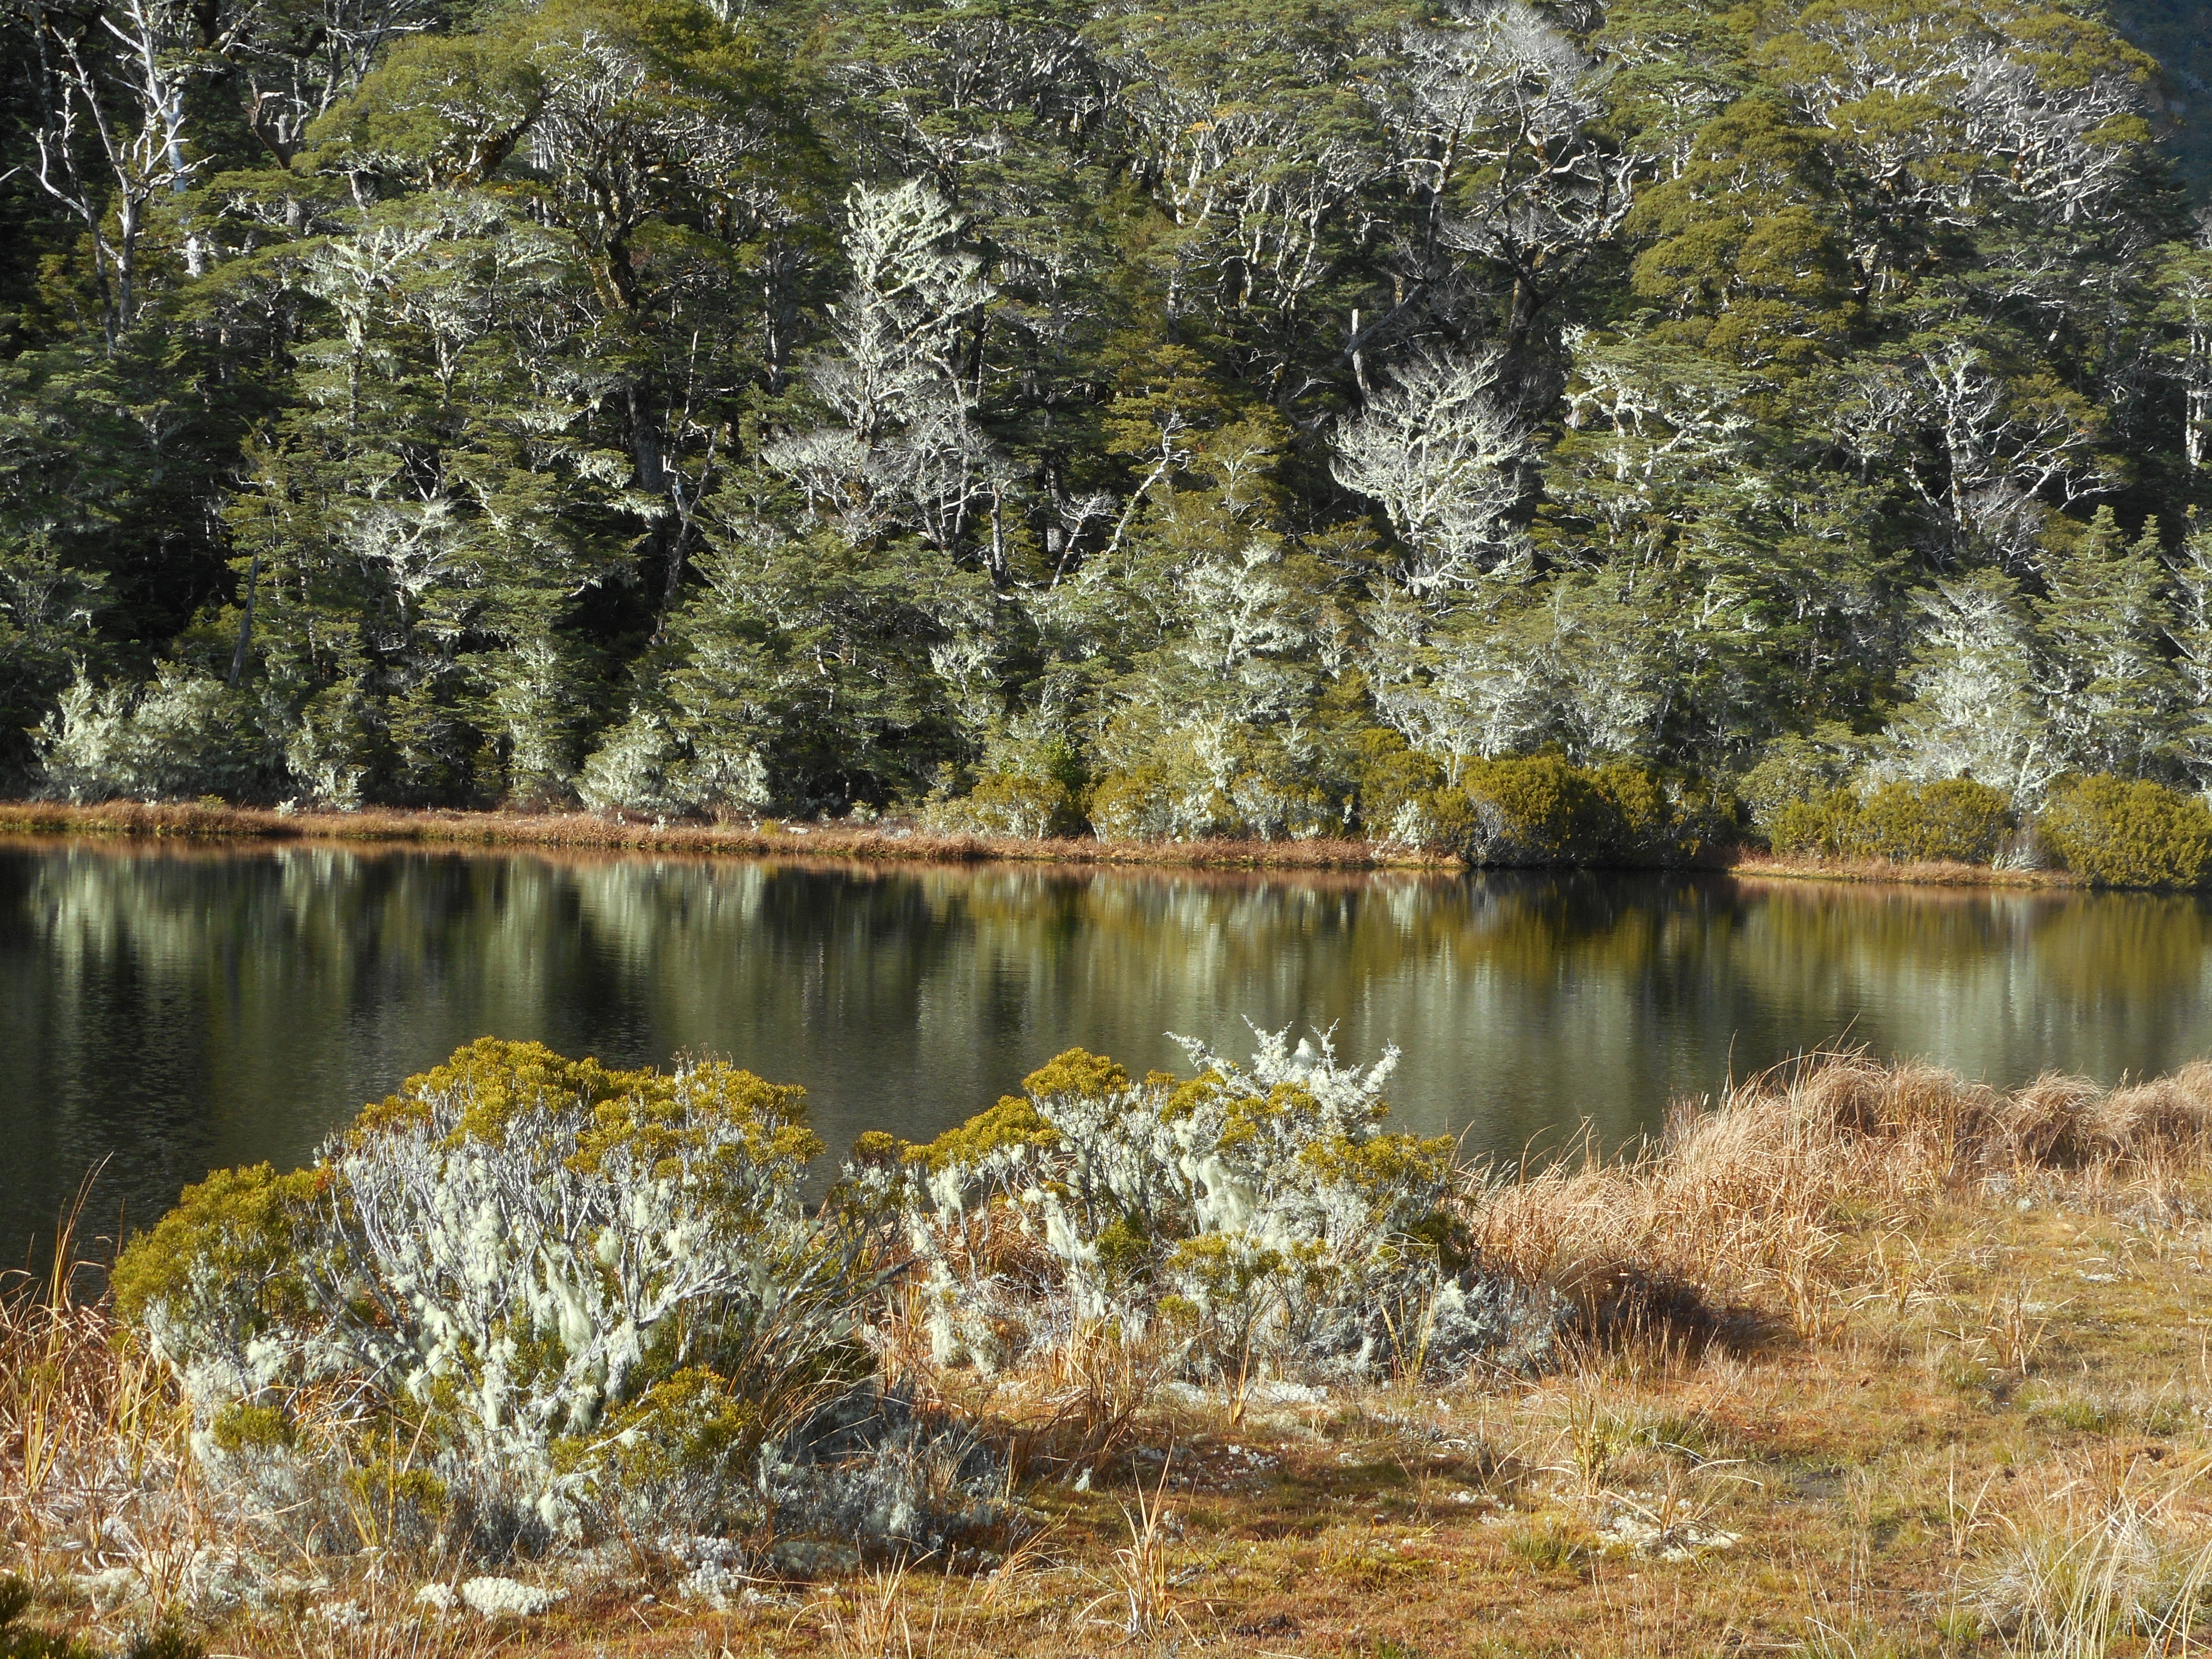
\includegraphics[width=9.5cm]{CannibalGorgeBridge11May2017Photo1}
\end{flushleft}
\end{minipage}
\begin{minipage}{.45\linewidth}
\begin{flushright}
    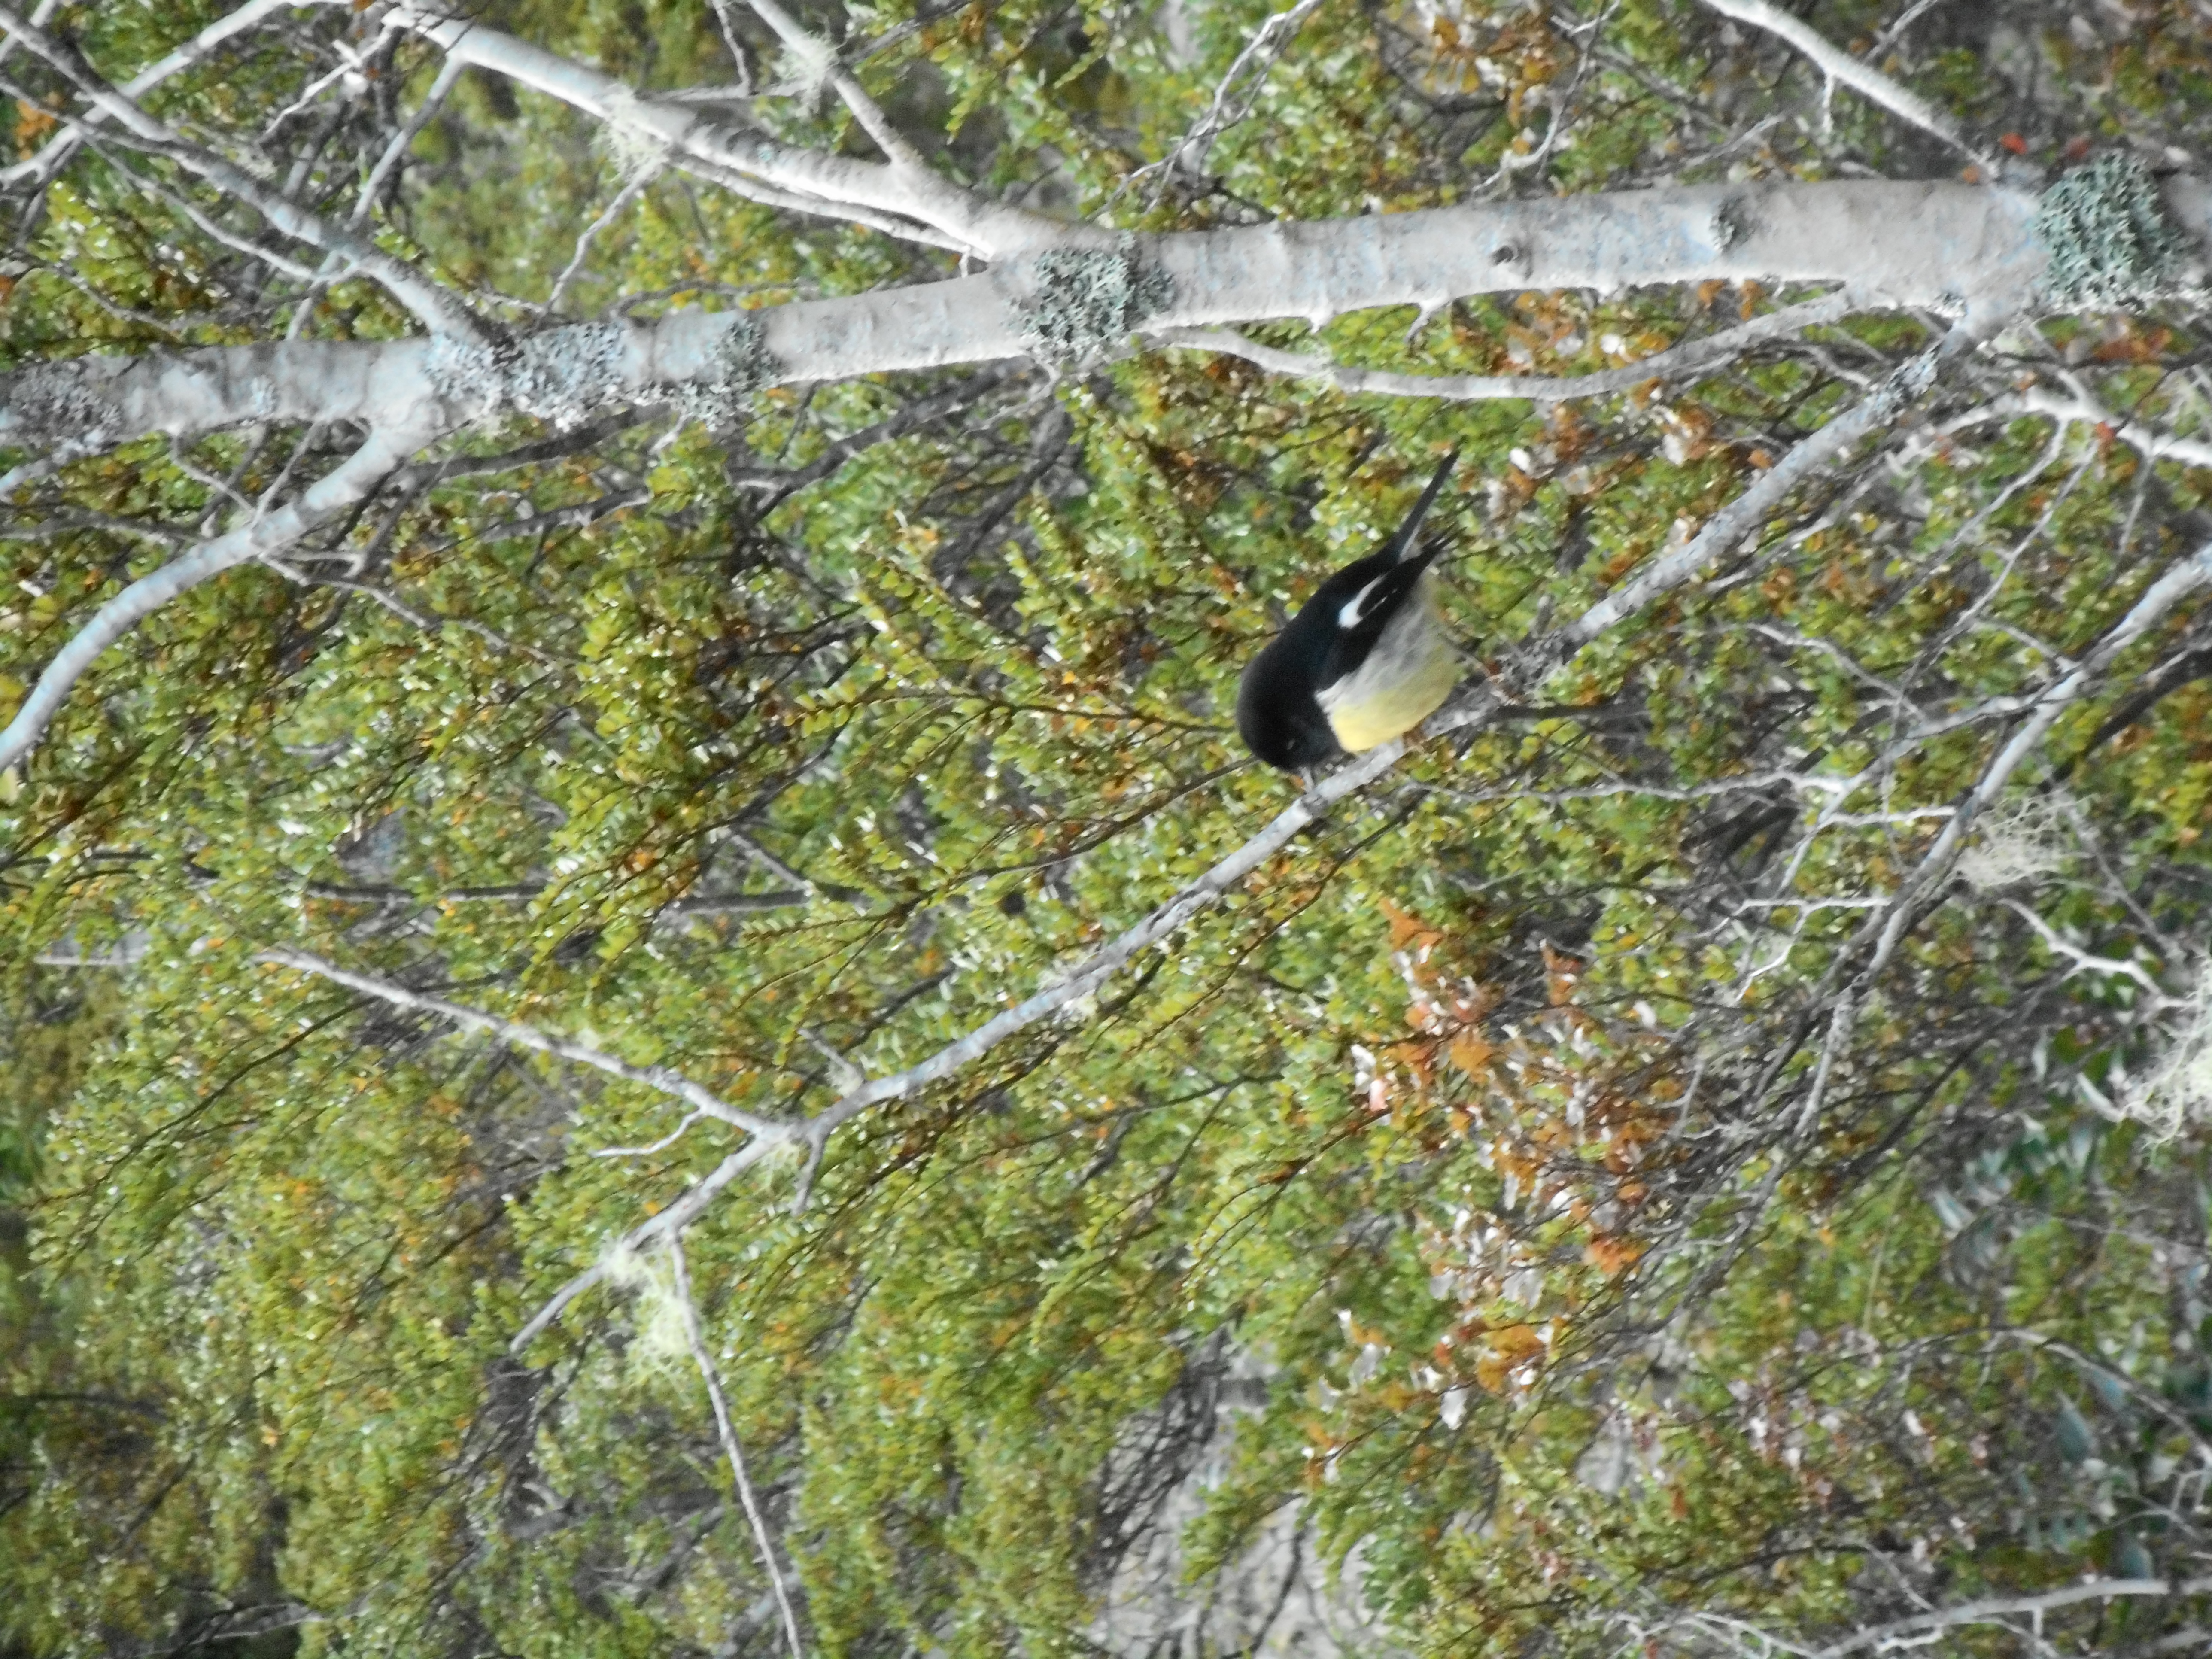
\includegraphics[width=9.5cm, angle=270]{CannibalGorgeBridge11May2017Photo2}
\end{flushright}
\end{minipage}
\end{figure}

\begin{flushright}
Ruth, Pierre, Robyn, Peter and dog
\end{flushright}

\end{document}
